\section{Architektur}

Das CCTD-Projekt ist Netzwerk-Applikation, welche aus zwei Hauptteilen besteht: Das effektive Spiel und eine Server-Komponente, welche die Lobby zur Verfügung stellt und alles andere, was für die Initialisierung eines Spieles nötig ist. Die Server-Komponente muss unabhängig von der Spiel-Komponente sein, damit Erweiterung am Server einen minimalen Einfluss auf das Spiel selber hat und damit in einem späteren Schritt dediziert gestart werden kann. Es handelt sich somit um einen Fat-Client. \\
Es ist im Allgemeinen angebracht, dass ein solches System auf dem Schichten-Model aufbauen sollte. Dies ist eine starke Unterstützung, um die Komplexität des System zu reduzieren und so minimal komplexen Programmcode zu erhalten. Moderne System werden in der Regel in 3 Schichten aufgeteilt: UserInterface, Domain, Logic.

\subsection{Logische Architektur}
\addcontentsline{lof}{figure}{Logische Architektur}
\begin{figure}[htb]
 \begin{center}
  \leavevmode
  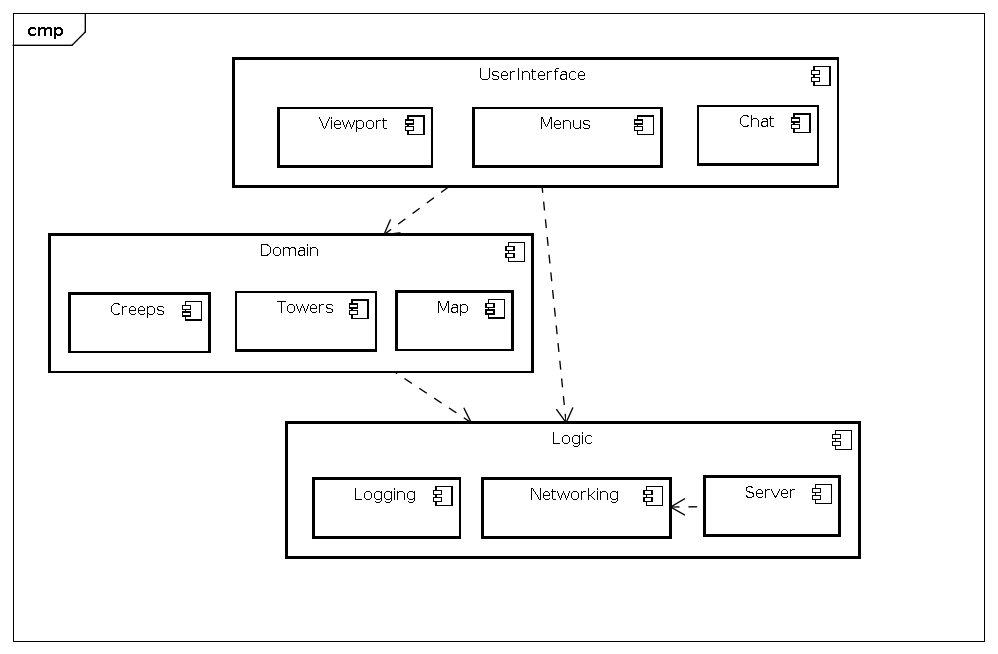
\includegraphics[width=0.95\textwidth]{logische_architektur.png}
 \end{center}
 \label{fig:logische_architektur}
\end{figure}
\addcontentsline{lot}{table}{Beschreibung: Logische Architektur}
\begin{longtable}{ | l | p{12cm} | }
 \hline
 \multicolumn{2}{|c|}{\textbf{UserInterface}} \\
 \hline
 \textbf{\glossary{name={Viewport}, description={Virtuelles Fenster für den Benutzer wodurch sie/er einen Bereich des Spiels sieht}}{Viewport}} & Zeichnet und definiert den sichtbaren Teil der Karte. \\
 \\
 \textbf{Menus} & Bietet Aktionen (Build,Upgrade,...) während dem Spiel an. \\
 \textbf{Chat} & UI-Elemente für den Spieler-Chat. \\
 \hline
 \multicolumn{2}{|c|}{\textbf{Domain}} \\
 \hline
 \textbf{\glossary{name={Creep}, description={gegnerisches Monster, welches abgeschossen werden soll}}{Creep}s} & Alle Arten von Creeps. \\
 \textbf{Towers} & Alle Arten von Towers inklusive ihren Upgrade Möglichkeiten. \\
 \textbf{Map} & Die Karte und alle Elemente, die sich direkt auf die Karte beziehen. \\
 \hline
 \multicolumn{2}{|c|}{\textbf{Logic}} \\
 \hline
 \textbf{Logging} & Bietet eine einheitliche Logging-Schnittstelle für die gesamte Applikation. \\
 \textbf{Networking} & Stellt eine Schnittstelle für die Kommunikation mit physikalisch entfernten Teil der Applikation zur Verfügung. \\
 \textbf{Server} & Beobachtet und Kontrolliert den Spielablauf, bietet eine Lobby \\
 \hline
\end{longtable}

